\chapter{欧氏空间中的Plateau问题}
\newcommand{\FG}{{\mathcal{F}_\gamma}}
\newcommand{\AG}{{\mathbb{A}_\gamma}}
\renewcommand{\EG}{{\mathbb{E}_\gamma}}
\renewcommand{\E}{{E}}
\renewcommand{\D}{{\mathbb{D}}}
\newcommand{\EE}{{\mathbb{E}}}
\renewcommand{\AA}{{\mathbb{A}}}
\newcommand{\PTT}[1]{{\partial_\theta #1}}
\newtheorem*{plateauproblem*}{Plateau问题}
\section{The Disk Case}
本章中, 我们回到最开始的问题:
\begin{plateauproblem*}
    给定简单闭曲线$\gamma \subset \R^3$, 是否存在以$\gamma$为边界的面积最小的曲面? 即, 寻找曲面$\Sigma, \partial \Sigma = \gamma$, 使得对于任意满足$\partial \Sigma' = \gamma$的曲面$\Sigma'$, 都有
    \begin{equation*}
        \Area(\Sigma) \le \Area(\Sigma')
    \end{equation*}
\end{plateauproblem*}
在本章, 按照Douglas和Rado的方法, 我们将给出Plateau问题的肯定的回答. 关于Douglas在Plateau问题上的工作的简介, 可以参考\cite{WorkofDouglas}.
\par 设$\gamma \subset \R^3$是简单闭曲线. 记
\begin{equation}
    \begin{split}
        \FG=\{
            u \mid  u\in C(\overline{\D})\cap W_{loc}^{1,2}(\D,\R^3),
            u\mid_{\P \D}: \P \D \to \gamma \text{是单调映射}.
        \}
    \end{split}
\end{equation}
\begin{remark}
    称$u\mid _{\P \D}$是单调映射, 是指我们将$\gamma$沿任意点剪断后看作实轴上的一段线段,  $u$是通常意义下的单调映射.  这里之所以没有要求$u$是同胚, 是因为同胚在求极限后(一致收敛拓扑)不会被保持,  而单调性总是会被保持的. 
\end{remark}
解决Plateau问题的第一选择是:取$u_k \in \FG$使得$\Area(u_k(\D)) \to \AG$, 并证明$\{u_k\}$存在收敛子列. 然而这种思路有两个问题需要解决:
\begin{enumerate}
    \item 我们可以改变$u_k$在任意点$p$附近的值, 得到$\tilde{u}_k$, 使得$\tilde{u}_k$与$\tilde{u}_k(\mathbb{D})$与 $u_k(\D)$相差"细长"的管状区域, 如图. 这样得到的$\tilde{u}_k$仍然是面积最小的列. 但是这样的列无法在通常的意义下收敛.  如图\eqref{figure_area_minimizing}所示.
    \begin{figure}[ht]
        \centering
        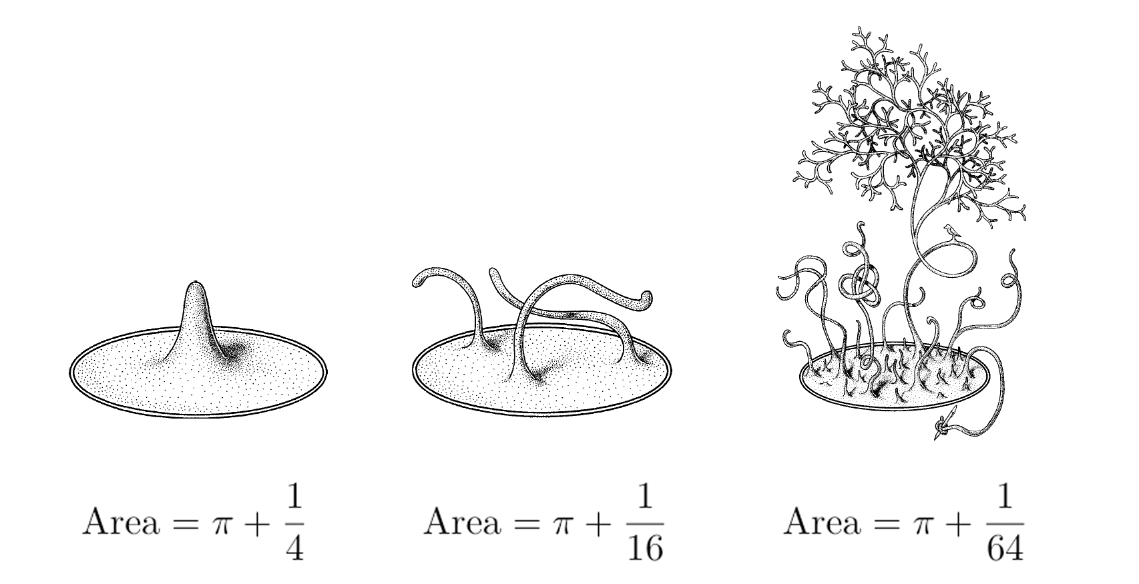
\includegraphics[scale=0.7]{images/area_minimizing.png}
        \caption{面积最小列, 但是没有收敛子列. 图片取自\cite{Morgan}}
        \label{figure_area_minimizing}
    \end{figure}
    \item 第二个问题是面积泛函是与参数选取无关的, 这意味着选取$\{u_k\}$后, 对于任意的微分同胚$\phi_k: \D \to \D$, $\Area(u_k\circ \phi_k(\D))= \Area(u_k(\D))$. 这种情况下, 我们也很难得到收敛子列.
\end{enumerate}
为了解决上面的问题, 我们将使用能量泛函而不是面积泛函. 当然, 首先我们需要说明的是, 对能量泛函求最小值和对面积泛函求最小值这两个问题是等价的(虽然对于能量泛函, 上述两个问题仍然存在, 但是我们较好的解决该问题的方法).
\begin{theorem} \label{rado_douglas}
    设$\gamma \subset \R^3$是可求长的Jordan曲线. 则存在映射$u \in \FG$使得 $\forall v \in \FG$, 
    \begin{equation}
        \Area(u(\D))\le \Area(v(\D)).
    \end{equation}
\end{theorem}
对于任意$u \in \FG$, 其面积与能量分别定义为
\begin{align}
    &\Area(u)=\int_\D\abs{u_x\wedge u_y} \\
    &\E(u)=\frac{1}{2}\int_\D\abs{u_x}^2+\abs{u_y}^2
\end{align}
简单计算可知
\begin{equation}\label{AleE}
    \Area(u)=\int_\D \sqrt{\abs{u_x}^2\abs{u_y}^2-\inner{u_x}{u_y}^2} \le \frac{1}{2}\int_\D \abs{u_x}^2+\abs{u_y}^2 \le\E(u).
\end{equation}
并且等号成立, 当且仅当$\abs{u_x}=\abs{u_y}, \inner{u_x}{u_y}=0$.
\par 记
\begin{align}
    &\AG=\inf\{\Area(v)\mid v \in \FG\}.\\
    &\EG=\inf \{\E(v)\mid v \in \FG\}.
\end{align}
\begin{definition}
    如果$u \in W^{1,2}(\mathbb{D},\R^3)$几乎处处满足$\inner{u_x}{u_y}=0$并且$\abs{u_x} = \abs{u_y}$, 则称$u$是几乎共形的.
\end{definition}
\begin{lemma}\label{ageg}
    $\AG=\EG$, 并且如果$u \in \FG$取到$\EG$, 则$u$是几乎共形的.
\end{lemma}
\begin{proof}
    由不等式\eqref{AleE}可知, $\AG \le \EG$.
    \par 对于反方向的, 设$u\in \FG$ 且$\Area(u) \le \AG + \epsilon$. 首先设$u$是浸入, 即$du$处处非退化. 设$(\D,g)$为$u$作用下的拉回度量, 即$g=du^*dx^2$, 由等温坐标的存在性可知, 存在光滑同胚$\phi: \D \to \D$使得$\phi$是$\mathbb{D} \to (\D,g)$ 之间的共形映射, 即$d\phi ^* g=\lambda^2dx^2$. 而$u\circ \phi$是共形浸入, 则有
    \begin{equation}
        \AG+\epsilon\ge \Area(u)=\Area(u\circ \phi)=\E(u\circ \phi) \ge \EG
    \end{equation}
    如果$du$有奇点, 那么我们定义$u^s: \D \to \R^5$, $u^s(x,y)=(u,sx,sy)\in \R^5$. 则$du^s$是非退化的. 像上面一样, 通过$u^s$拉回的度量为$du^*g_{\R^3}+s^2(dx^2+dy^2)$. 显然地, 
    \begin{equation}
        \Area(u^s)=\int_\D \det (du^*g_{\R^3}+s^2I)  \to \Area(u).
    \end{equation}
    \begin{equation}
        \E(u^s\circ\phi)=\int_\D \abs{(u^s\circ \phi)_x}^2+ \abs{(u^s\circ \phi)_y}^2 =\E(u\circ \phi)+s^2\E(\phi).
    \end{equation}
    因此, 当$s$足够小时, 我们有
    \begin{equation}
        \begin{split}
            \AG+2\epsilon \ge \Area(u)+\epsilon & \ge \Area(u^s\circ \phi)  \\
            &= \E(u^s\circ \phi)  \to \E(u\circ \phi) \\
            &\ge \EG.
        \end{split}
    \end{equation}
    若$E(u)=\EG$, 则$E(u)= \EG = \AG \le \Area(u)$, 则$E(u)=\Area(u)$. 由不等式\eqref{AleE}可知, $u$是几乎共形的.
\end{proof}
\begin{lemma}[Courant-Lebesgue引理] \label{courant_lebesgue}
    设$f \in W^{1,2}(\D,\R^3)$, $E(f) \le K$. 设$0 < \delta < 1$, $p \in \mathbb{D}$. 则存在$\rho \in (\delta, \sqrt{\delta})$ 使得$f\mid_{\P B(p,\rho) \cap \D}$是绝对连续的, 且$\forall z_1,z_2 \in \P B(p,\rho) \cap \D$, 成立 
    \begin{equation}
        \abs{f(z_1)- f(z_2)} \le (8K\pi)^{\frac{1}{2}}(\log \frac{1}{\delta})^{-\frac{1}{2}}.
    \end{equation}
\end{lemma}
\begin{proof}
    在$p$点处引入极坐标$(r,\theta)$. 由于$f \in W^{1,2}$, 则几乎对于所有的$r$, $f$关于$\theta$是绝对连续的.  则Cauchy不等式, 
    \begin{equation}
        \begin{split}
            \abs{f(z_1)-f(z_2)} &\le \int_{\P B \cap \D} \abs{f_\theta(re^{i\theta})}d\theta \\
            & \le \sqrt{2\pi} (\int_{\P B\cap \D} f^2_\theta d\theta)^{\frac{1}{2}}.
        \end{split}
    \end{equation}
    而由于在极坐标下, $Df=f_r \P_r + \frac{1}{r^2}f_\theta \P_\theta$, 则
    \begin{equation}
        \int_{B \cap \D} (f_r^2 + \frac{1}{r^2}f_\theta^2)r drd\theta \le 2K.
    \end{equation}
    取$\rho$使得$\int_{\P B \cap \D} f^2_\theta(\rho e^{i\theta})$取到(几乎)最小, 则有
    \begin{equation}
        \int^{\sqrt{\delta}}_\delta \int_{\P B \cap \D}\frac{1}{r^2}f^2_\theta(\rho e^{i\theta}) rd\theta dr \le 2K.
    \end{equation}
    因此, 
    \begin{equation}
        \abs{f(z_1)-f(z_2)} \le \sqrt{2\pi} \frac{2K}{ \int^{\sqrt{\delta}}_\delta \frac{1}{r}} = \sqrt{8K\pi}(\log \frac{1}{\delta})^{-\frac{1}{2}}.
    \end{equation}
\end{proof}
\begin{lemma}\label{three_point}
    设$p_1,p_2,p_3  \in \partial \D$是三个不同的点. 则对于任意三个点$\forall p'_1, p'_2, p'_3$, 存在唯一的共形同胚$\alpha: \D \to \D$使得$\alpha(p_i)=p'_i$. (假设$p_i, p'_i$在$\P \D$上都按逆时针排列)
\end{lemma}
\begin{proof}
    见任意复分析教材.
\end{proof}
\begin{lemma}\label{cut_curves}
    设$\gamma \subset \R^3$长度有限, 则$\forall \epsilon > 0$, 存在$\lambda>0$使得$\forall p,q \in \gamma$, 如果$d(p,q)< \lambda$, 那么$\gamma-\{p,q\}$的两条曲线中, 只有一条的直径(作为集合的直径)可以大于$\epsilon$. 
\end{lemma}
\begin{proof}
    略.
\end{proof}
现在, 固定三个点$p_i \in \P D$, $q_i \in \gamma$. 设$K > 0$, 记
\begin{equation}
    \FG^K=\{u \in \FG\mid E(u) \le K, u(p_i)=q_i\}.
\end{equation}
\begin{lemma} \label{boundary_equicontinuous}
    $\FG^K\mid_{\P D}$是等度连续的.
\end{lemma}
\begin{figure}[ht]
    \centering
    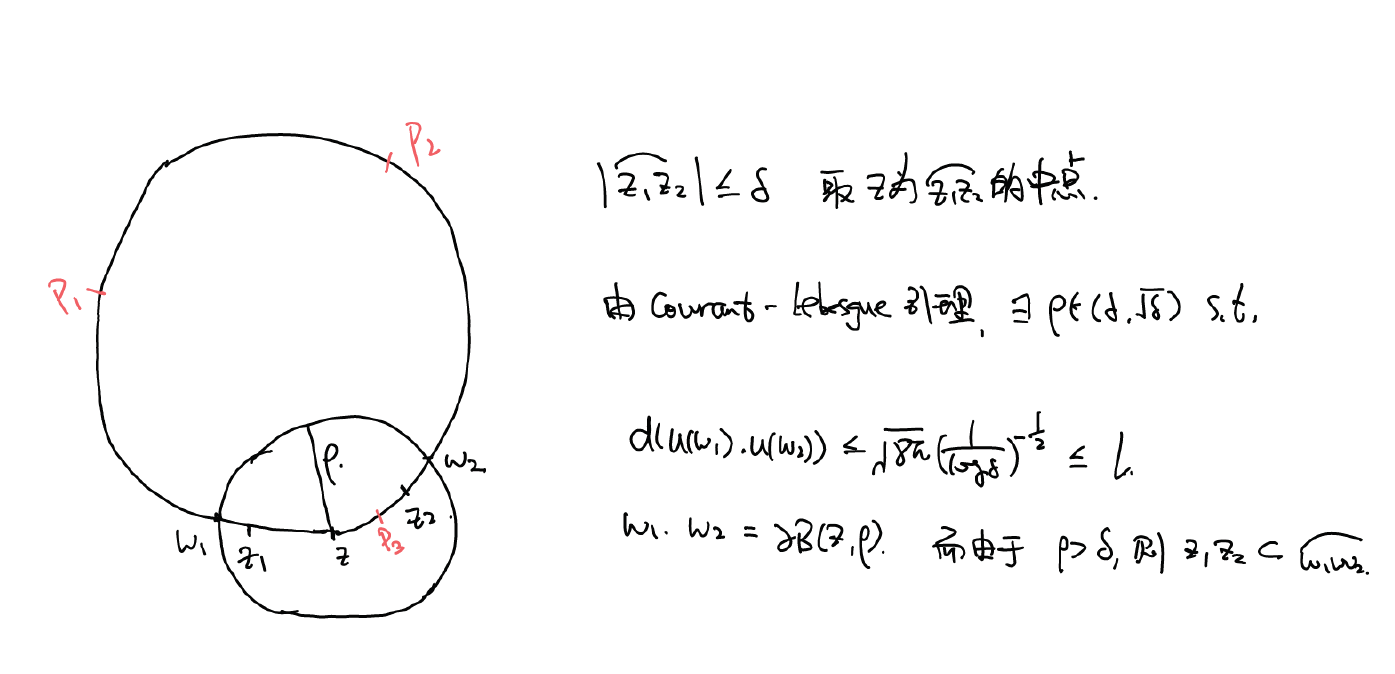
\includegraphics[scale=0.5]{images/courant_lebesgue.png}
    \caption{边界等度连续性}
    \label{equi_continuous}
\end{figure}
\begin{proof}
    我们选取$\epsilon$非常小, 使得$\gamma$中任意长度为$\epsilon$的曲线段都至多包含$\{q_i\}$中的一个点. 现在, 我们证明存在$\delta>0$, 使得如果$z_1,z_2 \in \P \D, \abs{z_1-z_2} \le \delta$, 则$\forall u \in \FG^K$, $\abs{u(z_1)-u(z_2)} \le \epsilon$.  
    \par 取$\delta$使得$(8K\pi)^{\rec{2}}(\log \rec{\delta})^{-\rec{2}} \le \lambda$, $\lambda$由引理\eqref{cut_curves}得到.  设$z_1,z_2 \in \P \D$.  设$\abs{z_1-z_2} \le \rec{\pi} \delta$, 用$\widehat{z_1z_2}$表示$\P \D - \{z_1,z_2\}$中较短的弧, 显然地, $\abs{\widehat{z_1z_2}} \le \delta$. 只要取$\delta$足够小, 就可以假设$\widehat{z_1z_2}$至多包含$\{p_i\}$中的一个点. 设$z$是弧$\widehat{z_1z_2}$的中点. 由引理\eqref{courant_lebesgue}, 存在$\rho \in (\delta, \sqrt{\delta})$使得$\forall u \in \FG^K$, 
    \begin{equation}
        d(u(w_1),u(w_2)) \le (8K\pi)^{\rec{2}}(\log \rec{\delta})^{-\rec{2}} \le \lambda.
    \end{equation}
    记$\{w_1,w_2\} = \P B(z,\rho) \cap \P \D$, 那么$u(w_1), u(w_2)$将$\gamma$分成两段, 其中较短的一段至多包含$\{q_i\}$中的一个点. 那么, 这一段的原像必定是$\widehat{w_1w_2}$.  而由于$\rho > \delta$, 则$z_1,z_2 \in \widehat{w_1w_2}$. 则$d(u(z_1),u(z_2)) \le \epsilon$.
\end{proof}
\begin{proof}[定理\eqref{rado_douglas}的证明]
    取$u_k \in \FG$ 且$E(u_k) \to \EG$. 由引理\eqref{three_point}, 存在$\phi_k$使得$u_k\circ \phi_k \in \FG^K$. 仍将$u_k\circ \phi_k$记为$u_k$.  用与$u_k$具有相同边界的调和函数替换$u_k$, 仍然记为$u_k$, 由于调和函数是能量最小的, 我们仍然有$E(u_k) \to \EG$.  由于$u_k$是调和的, 则
    \begin{equation}
        \max_{\D}\abs{u_k - u_l} = \max_{\P \D} \abs{u_k-u_l}.
    \end{equation}
    而根据引理\eqref{boundary_equicontinuous}, $u_k\mid_{\P \D}$ 包含一致收敛子列, 则$u_k$包含一致收敛子列. 设$u_k \to u$.  再选取$u_k$的子列, 使得$u_k \overset{\text{弱}W^{1,2}}{\longrightarrow} u$且$u_k \overset{L^2}{\longrightarrow} u$. 则由能量的下半连续性, 
    \begin{equation}
        E(u) \le \liminf E(u_k) \to \EG.
    \end{equation}
    最后, 由引理\eqref{ageg}, $\Area(u)=E(u)=\AG$.
\end{proof}
\ifcomment
    \begin{remark}
        如果没有三点正规化的话, 不影响等度连续性, 但是得到的极限可能是常值函数.
    \end{remark}
\fi
\section{The Annulus Case}
现在, 我们考虑复杂一点的情况. 设$\Gamma=\gamma_1 \cup \gamma_2$是两条简单闭曲线的并. 是否存在以$\Gamma$为边界的极小曲面?  
\par 与圆盘的情况不同的是,  并不总是能找到以$\Gamma$为边界的极小曲面.  这里我们给出一个反例.  设$\Sigma$为Catenoid, 即$\Sigma=\{\cosh^2 z = x^2+y^2\}$.  设$\Sigma_a= a\Sigma$.  那么, 当$a \to +\infty$时,  $\Sigma_a \to \emptyset$.  $a\to 0$时, $\Sigma_a \to 2\{z=0, x^2+y^2\ne 0\}$.  简单计算易知,  存在锥体$C_\lambda=\{x^2+y^2< \lambda^2z^2\}$使得$\forall \Sigma_a \cap C_\lambda = \emptyset$.  分别记$C^+_\lambda=C_\lambda \cap \{z>0\}$, $C^-_\lambda=C_\lambda \cap \{z<0\}$. 
\begin{figure}[ht]
    \centering
    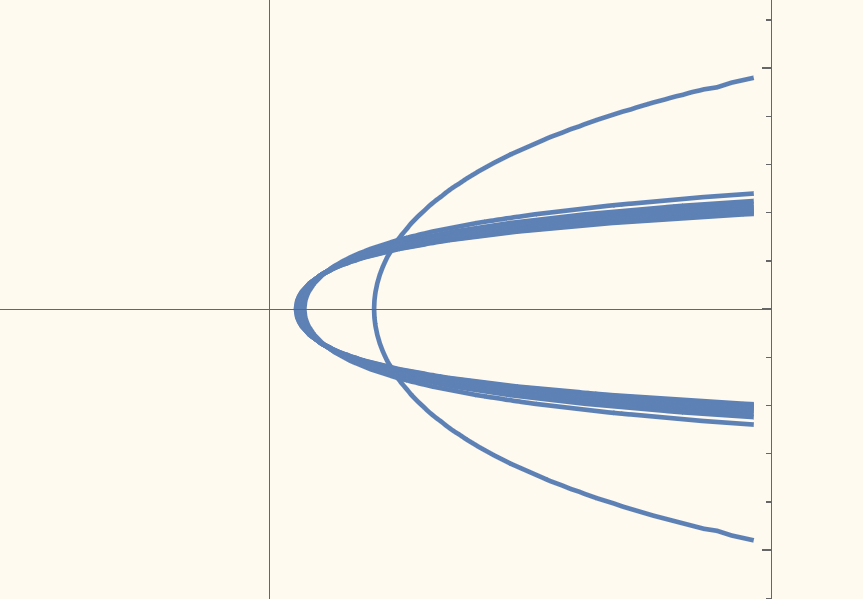
\includegraphics[scale=0.5]{images/sequence_of_catenoid.png}
    \caption{caption}
    \label{label}
\end{figure}
%\lstinputlisting[language=Mathematica]{mathematica/sequence_of_catenoid.m}
\begin{proposition}
    设$\Gamma=\gamma_1 \cap \gamma_2$, $\gamma_1 \subset C^+_\lambda, \gamma_2 \subset C^-_\lambda$. 则不存在以$\Gamma$为边界的有界连通极小曲面.
\end{proposition}
\begin{proof}
    设这样的极小曲面存在, 记为$M$.  显然地, $a \to 0$时,  $\Sigma_a \cap M \ne \emptyset$.  $a \to \infty$时, $\Sigma_a \cap M = \emptyset$. 那么存在$a$使得$\Sigma_a$恰好与$M$相切, 显然地这将与最大值原理矛盾.
\end{proof}

在此, 我们指出, 在解决给定拓扑型的Plateau问题时, 我们所会碰到的核心困难在于拓扑型的退化. 如图\eqref{annulus_minimizing}我们要寻找由两个圆盘围出的同胚于环面的极小曲面(图一图二均为两个环面, 且面积变小. 图三为两个圆盘). 当我们取面积递减的曲面序列的时候, 虽然所取的每一个曲面都同胚于环面, 但是最终得到的极限却是两个圆盘. 这种现象便是拓扑型的退化.即, 取极限后无法保证得到的曲面的拓扑是我们想要的.
\begin{figure}[ht]
    \centering
    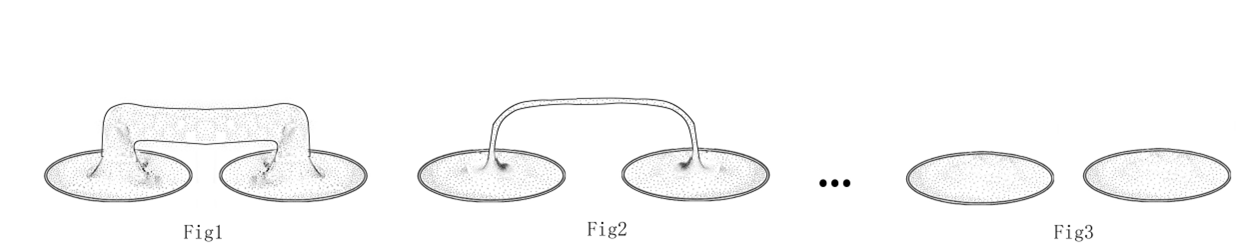
\includegraphics[scale=0.8]{images/annulus_minimizing.png}
    \caption{拓扑型的退化}
    \label{annulus_minimizing}
\end{figure}

\begin{lemma} \label{boundary_energy}
    设$\phi: \S^1 \to \R$是绝对连续的,  设$u\in C(\D)$是调和函数并且$u\mid_{\P \D}=\phi$. 则
    \begin{equation}
        \int_{\P \D} \abs{\nabla u}^2dxdy \le \int_{\S^1} \abs{\phi_\theta}^2d\theta.
    \end{equation}
\end{lemma}
\begin{proof}
    设$(r,\theta)$是极坐标. 设$c_n=\rec{2\pi}\int_{\S^1} \phi(\theta)e^{-i n \theta}d\theta$. 则$u, u_r$具有展开式
    \begin{align}
        &u(r,\theta)=\sum_{-\infty}^{+\infty}c_n r^{\abs{n}}e^{in\theta}, \label{fourier_u} \\
        &u_r(r,\theta)=\sum_{-\infty}^{+\infty}c_n\abs{n} r^{\abs{n}-1}e^{in\theta}. \label{fourier_ur}\\
    \end{align}
    由散度定理, 并将\eqref{fourier_u},\eqref{fourier_ur}代入计算可知
    \begin{equation}
        \begin{split}
            \int_{{\abs{z}\le r}}\abs{\nabla u}^2dxdy & =\int_{\{\abs{z}=r\}}uu_rd\theta\\
            &=2\pi \sum_{-\infty}^{+\infty}\abs{n}r^{2n}\abs{c_n}^2.
        \end{split}
    \end{equation}
    另外, 有
    \begin{equation}
        \int_{\S^1} \abs{u_\theta}^2 = 2\pi\sum_{-\infty}^{+\infty} \abs{n}^2\abs{c_n}^2.
    \end{equation}
    令$r \to 1$即可.
\end{proof}
\begin{lemma} \label{fill_hole}
    设 $\delta <1$. 定义
    \begin{equation}
        \eta(r)=\left\{
            \begin{aligned}
                &1 \s r \ge \sqrt{\delta}, \\
                &1+\frac{\log \sqrt{\delta}- \log r}{ \log \sqrt{\delta}} \s \delta \le r \le \sqrt{\delta}\\
                &0 \s r \le \delta
            \end{aligned}
            \right.
    \end{equation}
    设$u \in W^{1,2}(\Sigma) \cap C(\Sigma)$. 定义
    \begin{equation}
        u_\delta(z)=\left\{
            \begin{aligned}
                & u(z) \s d(u(z), p) \ge \sqrt{\delta} \\
                & p+ \eta(d(u(z),p))(u(z)-p)
            \end{aligned}
        \right.
    \end{equation}
    则当$\delta \to $时, $E(u_\delta) \to E(u)$.
\end{lemma}
\begin{figure}[ht]
    \centering
    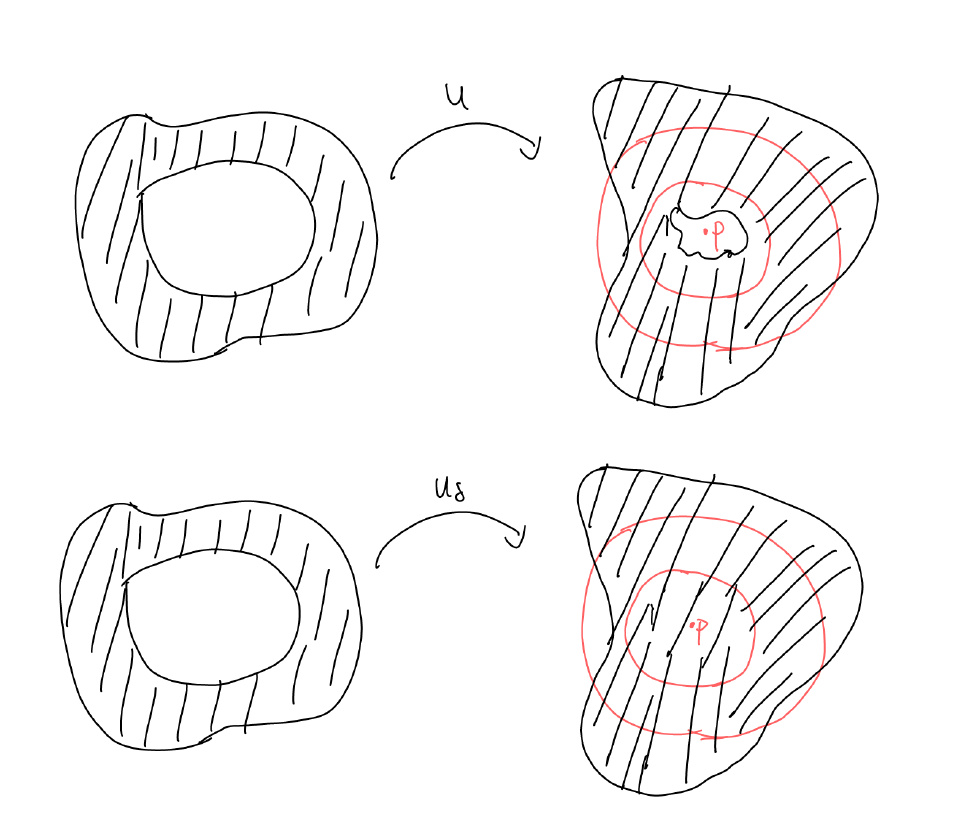
\includegraphics[scale=0.5]{images/contraction.png}
    \caption{$u_\delta$填补了$u$的像中的"空洞"}
    \label{aaaanonlabel}
\end{figure}
\begin{theorem}
    设$\Gamma= \gamma_1 \cup \gamma_2 \subset \R^3$是两条不相交的简单闭曲线的并. 设存在以$\Gamma$为边界的双连通曲面$M$使得
    \begin{equation} \label{douglas_condition_annulus}
        \Area(M) < \AG_{\gamma_1}+\AG_{\gamma_2}.
    \end{equation}
    则存在以$\Gamma$为边界的双连通的极小曲面.
\end{theorem}
\begin{proof}
    设$u_k: \Sigma \to \R^3$, $E(u_k) \to \EE_{\Gamma}$.  记$K=\EE_{\Gamma}+1 < +\infty$. 这里, $\Sigma_k = \S\times (0,s_n)$. 现在,我们证明: 存在子列使得 $s_n \to s >0$.  $\Sigma_n$上的参数记为$(\theta,r)$. $\theta \in \S^1, r \in (0,s_k)$.
    \begin{claim}
        $\{s_k\}$有严格正的下界.
        \begin{subproof}
            记$d=d(\gamma_1,\gamma_2)>0$. $\forall \theta$, 设$\alpha$ 为直线$\theta \times (0, s_k)$. 显然地, $l_{u_k(\alpha)} \ge d$. 则由Cauchy不等式
            \begin{equation}
                d^2 \le (\int^{s_k}_0 \abs{du_k \alpha'} ds)^2 \le s_k \int^{s_k}_0 (\PTT{u_k})^2dr.
            \end{equation}
            于是, 有
            \begin{equation}
                \frac{2\pi d^2}{s_k} \le \int_{\S^1}\int^{s_k}_0 (\PTT{u_k})^2 drd\theta \le E(h) \le K.
            \end{equation}
            则$s_k \ge \frac{2\pi d^2}{K}$.
        \end{subproof}
    \end{claim}
    \begin{claim}
        $\{s_k\}$有上界(不等于$+\infty$).
        \begin{subproof}
            反证法.  设$s_k \to +\infty$. 由于$\E(u_k) \le K$,  则存在$\rho_k \in (0, s_k)$使得
            \begin{equation}
                s_k\int_{\S^1} (\PTT{u_k})^2(\theta,\rho_k) d\theta \le K.
            \end{equation}
            则有$\int_{\S^1} (\PTT{u_k})^2(\theta,\rho_k) d\theta  \to 0$. 记$D_{\rho_k}=\D \times \{\rho_k\}$. 现在以$u_k(\rho_k,\theta)$为边界值, 由引理\eqref{boundary_energy}可知, 存在函数$f_k: \D_\{\rho_k\} \to \R^3$使得$E(f_k) \to 0$. 现在我们定义两个新的映射:
            \begin{equation}
                \tilde{u}_k^1: \S^1 \times (0,\rho_k) \cup \D_{\rho_k}\to \R^3.  \s  \tilde{u}_k^1=\left\{
                    \begin{aligned}
                        &u_k\s x \in \S^1 \times (0,\rho_k),\\
                        &f_k\s x \in \D_{\rho_k}.
                    \end{aligned}
                \right.
            \end{equation}
            \begin{equation}
                \tilde{u}_k^2: \S^1 \times (0,\rho_k) \cup \D_{\rho_k}\to \R^3.  \s  \tilde{u}_k^2=\left\{
                    \begin{aligned}
                        &u_k\s x \in \S^1 \times (\rho_k, s_k),\\
                        &f_k\s x \in \D_{\rho_k}.
                    \end{aligned}
                \right.
            \end{equation}
            则$E(\tilde{u}_k^1)+E(\tilde{u}_k^2) \le E(u_k)+2E(f_k)$. 而显然地, $\tilde{u}_k^1,\tilde{{u}}_k^2$的定义域都同胚于单位圆盘. 则
            \begin{equation}
                \begin{split}
                    \AA_{\gamma_1}+\AA_{\gamma_2} = \EE_{\gamma_1}+\EE_{\gamma_2} & \le  \lim E(\tilde{u}_k^1)+E(\tilde{u}_K^2)  \\
                    &\le \lim E(u_k) + 2E(f_k) \to \EE_\Gamma=\AA_\Gamma.
                \end{split}
            \end{equation}
            这与条件\eqref{douglas_condition_annulus}矛盾.
        \end{subproof}
    \end{claim}
    设$\Sigma_k \to \Sigma = \S^1 \times (0,s)$. 同时, 我们可以假设$u_k$定义在$\Sigma$上.
    \begin{claim}
        $u_k\mid_{\P \Sigma}$是等度连续的.
        \begin{subproof}
            我们只考虑$u_k\mid_{\P \D}$的等度连续性即可.  由引理\eqref{courant_lebesgue}, $\forall p \in \P \D, \delta>0$, 存在$\rho_k \in (\delta,\sqrt{\delta})$使得
            \begin{equation}
                l_{u_k(\P B(p,\rho_k) \cap \Sigma)} \le \sqrt{8K\pi}(\log(\rec{\epsilon}))^{-\rec{2}}.
            \end{equation}
            记$\beta=\P B(p,\rho_k)$将$\P \D$分成两部分. 其中短的一部分记为$C'$, 长的部分记为$C''$. $u_k(\beta)$将$\gamma_1$分成两部分, 其中短的记为$\gamma_1'$, 长的记为$\gamma_2'$. 由Courant-Lebesgue引理,  如果$u_k(C')=\gamma_1'$, 那么$u_k$是等度连续的.  反证法. 设$u_k(C')=\gamma_2''$. $u_k(C''\cup\beta)=u(\beta) \cup \gamma_1''$, 而$l_{u(\beta)\cup \gamma_1''} = \epsilon_k \to 0$. 取$q \in \R^3$使得$d(q, u_k(\beta) \cup \gamma_1'') < \epsilon_k$. 应用引理\eqref{fill_hole}, 得到新的映射$\tilde{u}_k$.
        \end{subproof}
    \end{claim}
\end{proof}
\section{The General Case}
\subsection{双曲几何}